\documentclass{beamer}

\usepackage[utf8x]{inputenc}
\usepackage[english,bulgarian]{babel}
\usepackage[export]{adjustbox}

\mode<presentation> {
	\usetheme{Berlin}
}

\usebackgroundtemplate {
	
\includegraphics[width=370px, height=270px, trim=0 0 0 -80px]{BackTriangles025.png}
}

\title[Конкурс на ИИКТ-БАН, София, България, 2019]{
	\small{Конкурс за заемане на академичната длъжност “главен асистент” по специалност „Информатика“, професионално направление 4.6. „Информатика и компютърни науки“, секция „Моделиране и оптимизация“ на ИИКТ-БАН, обявен в ДВ бр. 41 от 21.05.2019г.}
}

\author{инж. д-р Тодор Балабанов}

\date{02.IX.2019}

\institute[ИИКТ-БАН, МО] {
    Институт по информационни и комуникационни технологии  \\ 
	Българска академия на науките \\
	\medskip
	\textit{todorb@iinf.bas.bg}
}

\addtobeamertemplate{navigation symbols}{}{
    \usebeamerfont{footline}
    \usebeamercolor[fg]{footline}
    \hspace{1em}
    \insertframenumber/\inserttotalframenumber
}

\begin{document}

\begin{frame}
\titlepage
\end{frame}

\begin{frame}
\frametitle{Съдържание}
\tableofcontents
\end{frame}

\section{Въведение}

\begin{frame}
\center \huge{Въведение}
\end{frame}

\begin{frame}
\frametitle{инж. д-р Тодор Балабанов}
\begin{itemize}
  \item Програмист в секция "Моделиране и оптимизация" на ИИКТ-БАН
  \vspace{0.5cm}
  \item Доктор по "Информатика и компютърни науки"
  \item Бакалавър по "Компютърни системи и технологии"
  \item Магистър по "Софтуерни технологии в Интернет"
  \item Бакалавър по "Информатика"
  \item Специалист по "Програмно осигуряване"
\end{itemize}
\end{frame}

\begin{frame}
\frametitle{Дисертационен труд}
\begin{itemize}
  \item Тема: "Разпределена система за прогнозиране на времеви редове с еволюционни алгоритми и изкуствени невронни мрежи"
  \item Публикации:
  \begin{itemize}{\fontsize{1}{2}\selectfont
	  \item Балабанов Т., Занкински И., Симеонова В., Прогнозиране на времеви редове с изкуствени невронни мрежи и диференциална еволюция в разпределена среда, Работни статии на ИИТ, IIT/WP-268B, ISSN:1310-652X, 2010
	  \item Балабанов. Т., Прогнозиране с евристични подходи в разпределена среда, Proceedings of Anniversary Scientific Conference 40 Years Department of Industrial Automation, ISBN:978-954-465-043-8, 163-166, 2011
	  \item {\color{red}Balabanov. T., Zankinski I., Dobrinkova N., Time Series Prediction by Artificial Neural Networks and Differential Evolution in Distributed Environment, Large-Scale Scientific Computing, Lecture Notes in Computer Science, vol. 7116, ISBN:978-3-642-29842-4, 198-205, 2011}
	  \item Балабанов, Т., Избягване на локални оптимуми при евристични популационни алгоритми в разпределена среда, Сборник с доклади от XXII Международен симпозиум Управление на енергийни, индустриални и екологични системи, ISSN:1313-2237, 83 - 86, 2015
	  \item {\color{red}Balabanov, T., Zankinski, I., Barova, M.. Distributed Evolutionary Computing Migration Strategy by Incident Node Participation. Large-Scale Scientific Computing, Lecture Notes in Computer Science, 9374, Springer International Publishing Switzerland, ISBN:978-3-319-26520-9, 203 - 209, 2015}
	  \item Балабанов, Т., Генова, К., AJAX разпределена система за обучение на изкуствени невронни мрежи с еволюционни алгоритми, Сборник с доклади от XXIV Международен симпозиум Управление на топло енергийни обекти и системи, Управление на енергийни, индустриални и екологични системи, ISSN:1313-2237, 49 - 52, 2016
	  \item Balabanov T., Keremedchiev D., Goranov I., Web Distributed Computing For Evolutionary Training Of Artificial Neural Networks, International Conference InfoTech-2016, Varna - St. St. Constantine and Elena resort, Bulgaria, ISSN:1314-1023, 210-216, 2016
	  \item Балабанов, Т., Генова, К., Разпределена система за обучение на изкуствени невронни мрежи, базирана на мобилни устройства, Proceedings of International Conference Automatics and Informatics’2016, ISSN:1313-1850, 49 - 52, 2016
	}\end{itemize}
\end{itemize}
\end{frame}

\section{Разработка}

\begin{frame}
\center \huge{Разработка}
\end{frame}

\begin{frame}
\frametitle{Прогнозиране - технически анализ}
\begin{itemize}
	\item Финансови времеви редове (валутни двойки от FOREX)
	\item Търси се спад или повишаване на стойностите
	\item При възможност се търси и магнитуд
\end{itemize}
\end{frame}

\begin{frame}
\frametitle{Система за прогнозиране}
\begin{itemize}
	\item Класификатор на базата на изкуствени невронни мрежи
	\item Обучение на класификатора с еволюционни алгоритми
	\item Изчисления в разпределена среда
	\begin{itemize}
		\item Централен сървър на MySQL/PHP
		\item Мобилни устройства на Android
	\end{itemize}
\end{itemize}
\end{frame}

\begin{frame}
\frametitle{Развитие на съществуваща идея}
\begin{figure}[h]
  \centering
  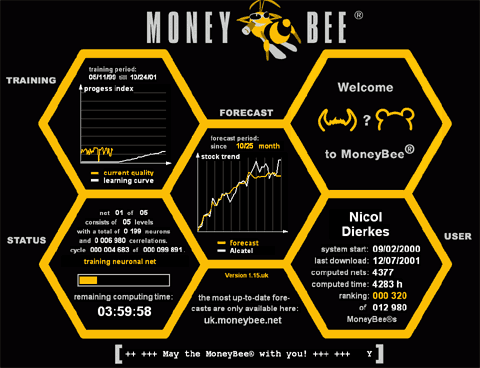
\includegraphics[width=0.8\textwidth]{Moneyb2.png}
\end{figure}
\end{frame}

\begin{frame}
\frametitle{Разпределена система}
\begin{figure}[h]
  \centering
  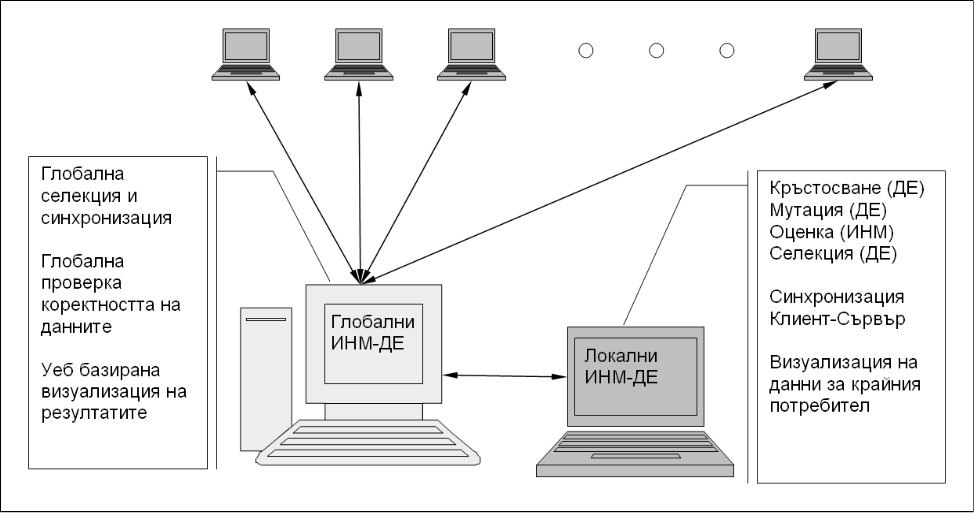
\includegraphics[width=\textwidth]{DistributedSystem.png}
\end{figure}
\end{frame}

\begin{frame}
\frametitle{Комуникация клиент-сървър}
\begin{figure}[h]
  \centering
  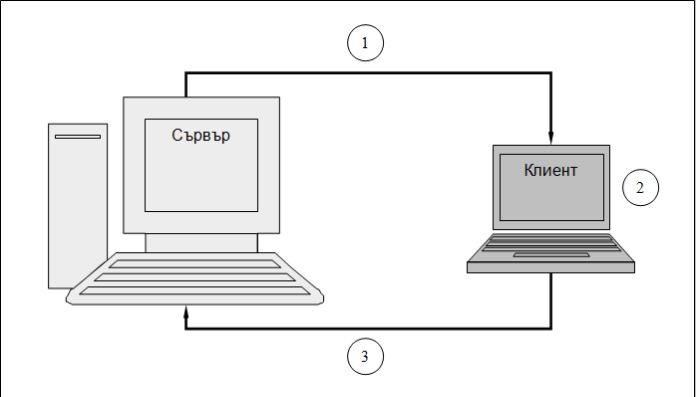
\includegraphics[width=\textwidth]{ClientServer.png}
\end{figure}
\end{frame}

\begin{frame}
\frametitle{Финансови данни}
\begin{figure}[h]
  \centering
  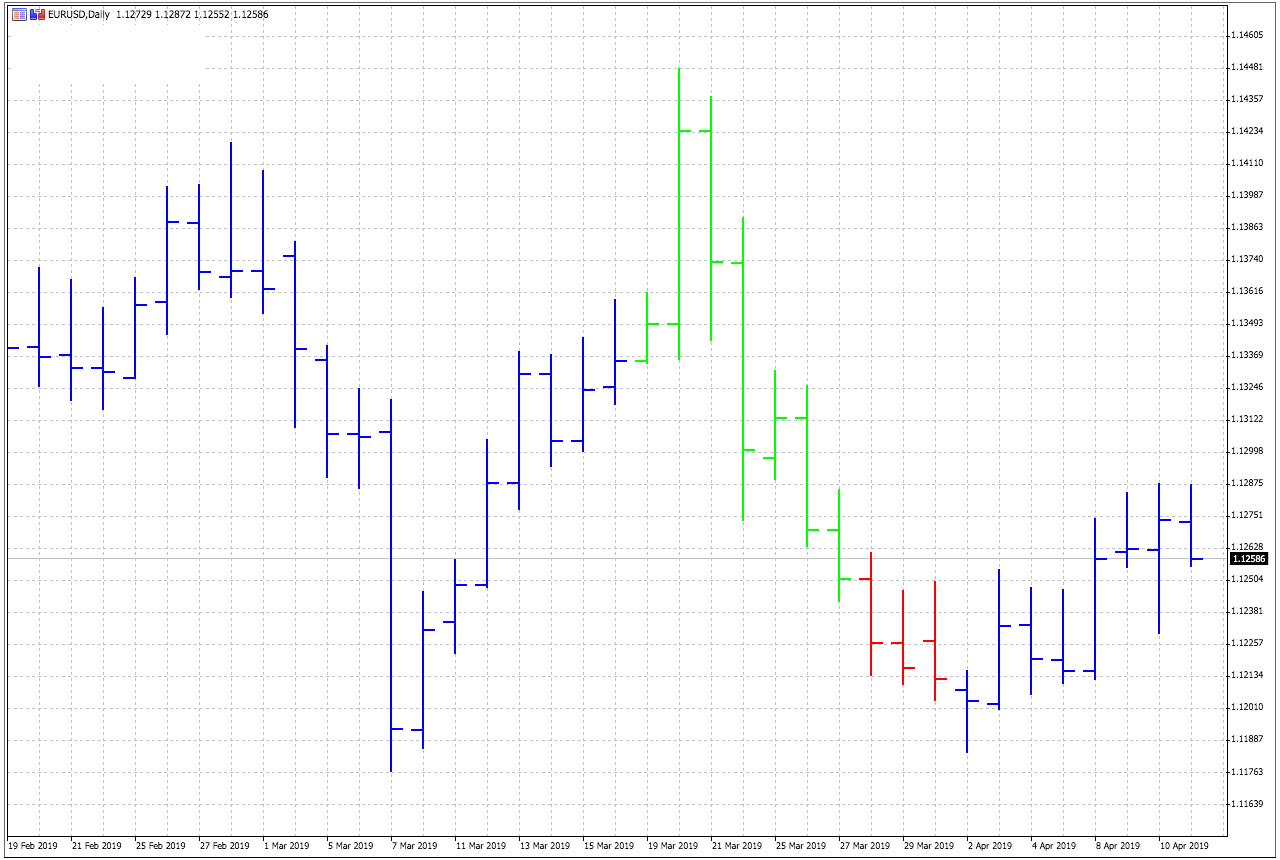
\includegraphics[width=0.9\textwidth]{ForexData.png}
\end{figure}
\end{frame}

\begin{frame}
\frametitle{Обработка в мобилното приложение}
\begin{figure}[h]
  \centering
  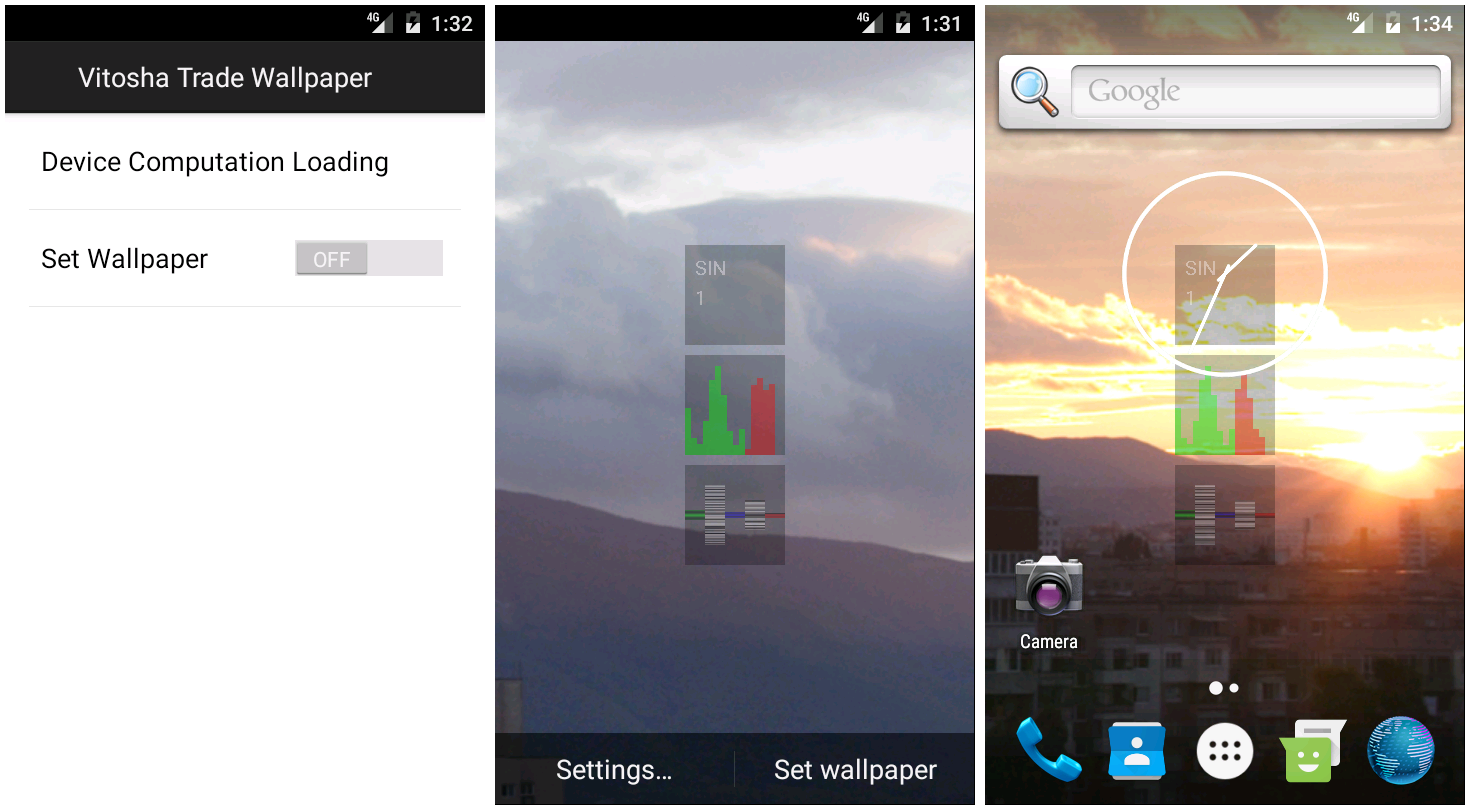
\includegraphics[width=\textwidth]{MobileClient.png}
\end{figure}
\end{frame}

\section{Заключение}

\begin{frame}
\center \huge{Заключение}
\end{frame}

\begin{frame}
\frametitle{Обобщение}
\begin{itemize}
	\item Силно недофинансирана дейност
	\item Малко и слабо подготвени кадри
	\item Ще отнемат значително количество време
\end{itemize}
\end{frame}

\begin{frame}
\frametitle{Въпроси и отговори}
\center \huge{Благодаря за вниманието!}
\end{frame}

\end{document}

